In figure~\ref{fig:slice-comparision}, a slice at $z=\SI{40}{nm}$ is compared to the simulation in ref.~\cite{heeg}. The overal local enhancement of the simulation nicely reproduces the simulation. The biggest difference is noticeable close to the outer edges of the nano dimer: Compared to the simulation from ref.~\cite{heeg} the enhancement is slightly bigger.

\begin{figure}[!h]
  \centering
  \begin{subfigure}{0.50\textwidth}
    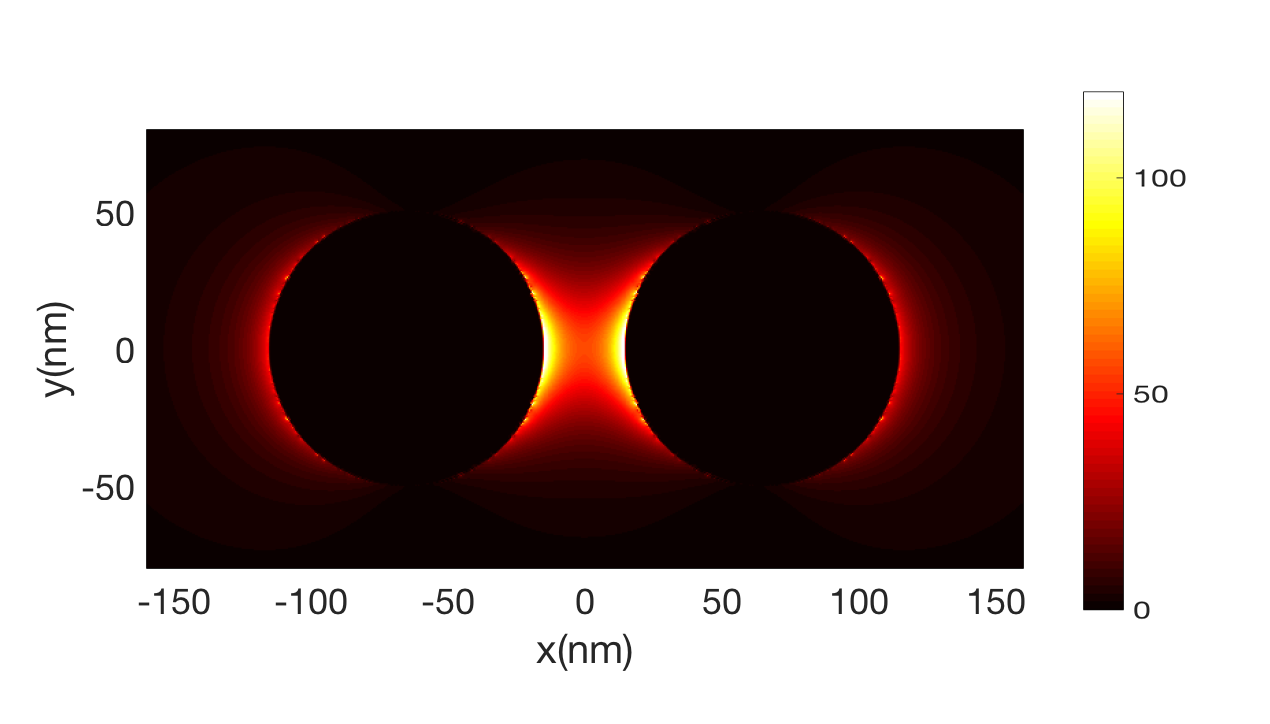
\includegraphics[width=\textwidth]{./images/40nm.png}
  \end{subfigure}
  ~
  \begin{subfigure}{0.40\textwidth}
    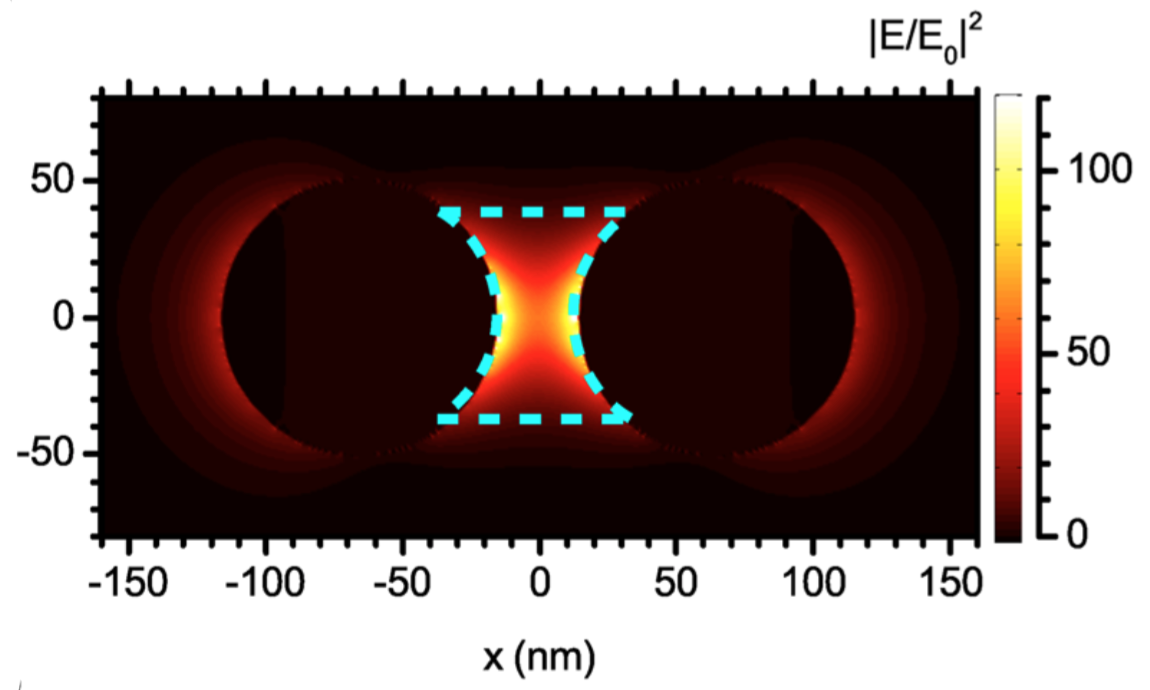
\includegraphics[width=\textwidth]{./images/local-enhancement-heeg.png}
  \end{subfigure}
  \caption{\textbf{(a)} Near field enhancement $|E/E_0|^2$ in the $xy$-plane at a height of $z=\SI{40}{nm}$. \textbf{(b)} Simulation from ref.~\cite{heeg}.}
  \label{fig:slice-comparision}
\end{figure}

This difference is also noticeable by plotting the near field enhancement at $z = \SI{40}{nm}, y = \SI{0}{nm}$ as a function of $x$ (figure \ref{fig:yline}). The graph reproduces the simulation of ref.~\cite{heeg} well within the dimer cavity, with a maximum enhancement of $100$ at the edges of the cavity and a minimum enhancement of $50$ in the cavity center. The biggest difference is visible at the outer edges of the gold nano dimer.

\begin{figure}[!h]
  \centering
  \begin{subfigure}{0.45\textwidth}
    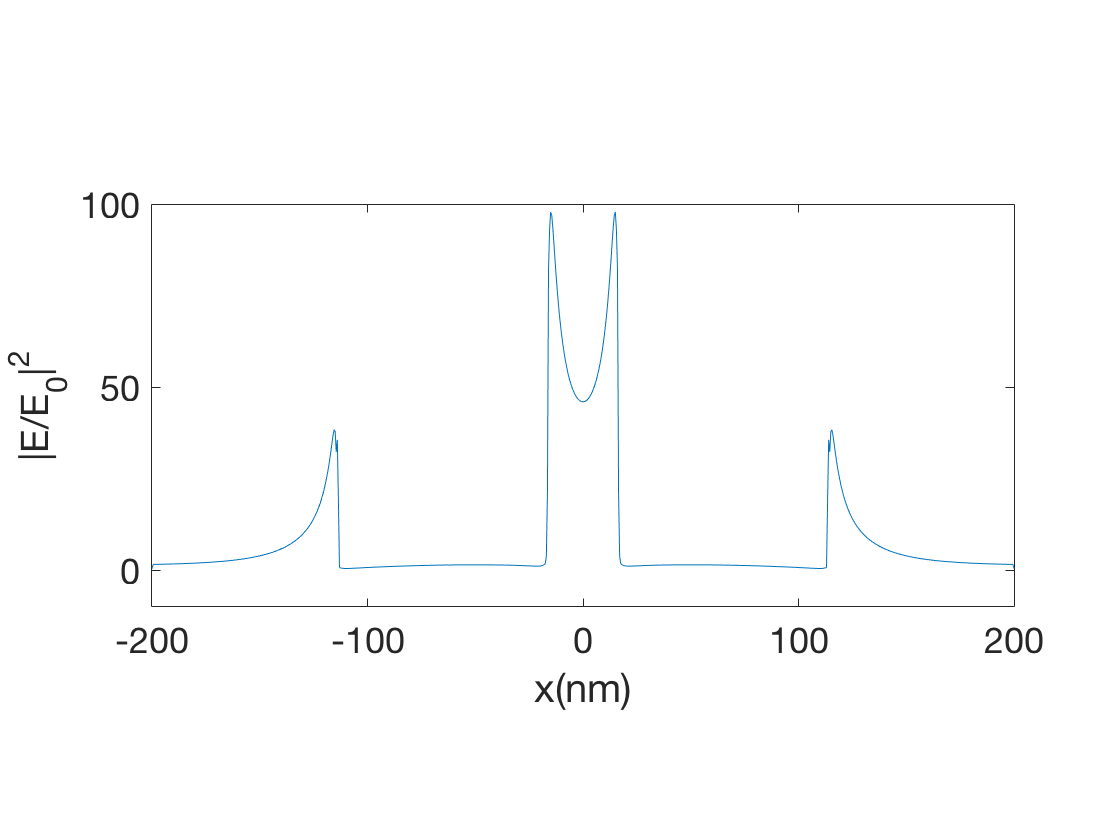
\includegraphics[width=\textwidth]{./images/40nm-y.png}
  \end{subfigure}
  ~
  \begin{subfigure}{0.45\textwidth}
    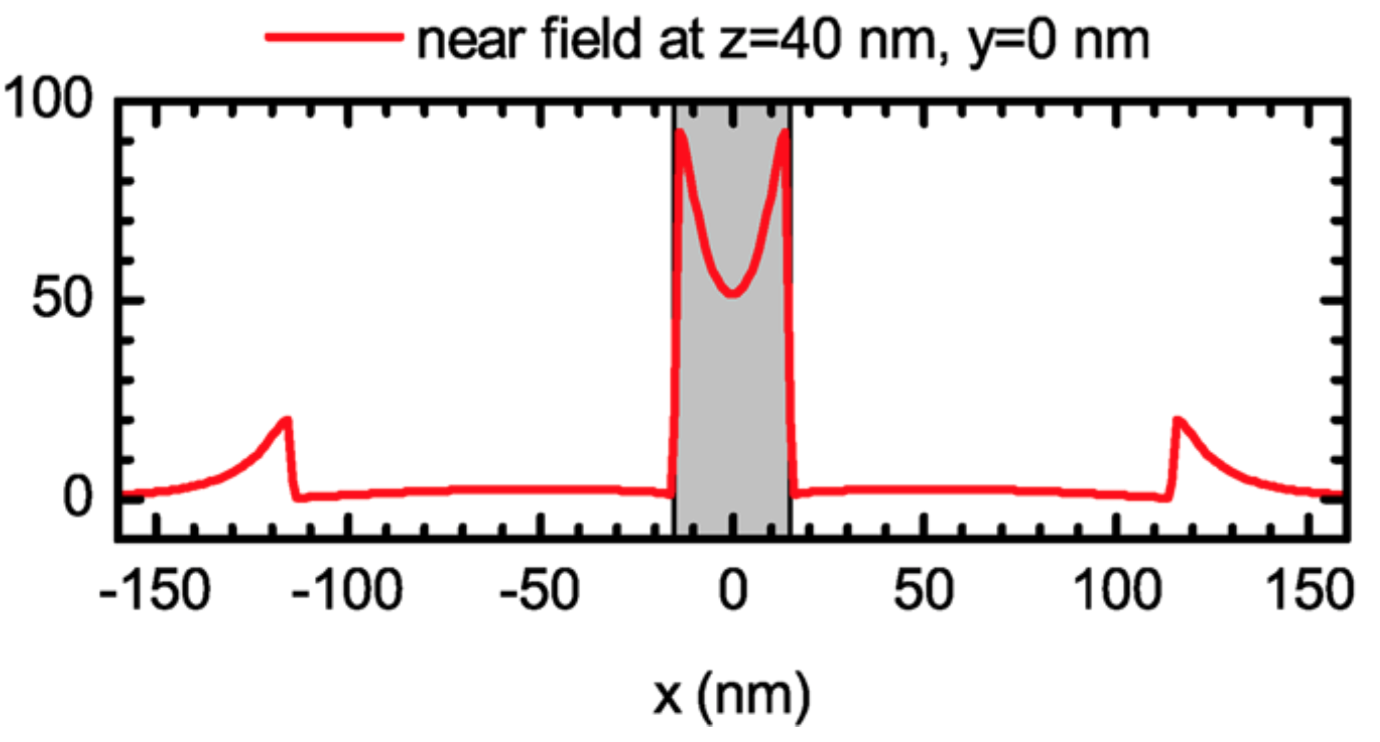
\includegraphics[width=\textwidth]{./images/heeg-y-line.png}
  \end{subfigure}
  \caption{\textbf{(a)} Near field enhancement $|E/E_0|^2$ at $z = \SI{40}{nm}, y = \SI{0}{nm}$ as a function of $x$. \textbf{(b)} Original results by \cite{heeg}.}
  \label{fig:yline}
\end{figure}

These differences can be explained with the different corner radii where sharper edges lead to a stronger enhancement. However, because the  enhancement outside the cavity can be neglected compared to the enhancement within the cavity according to \cite{heeg}, the results of the simulation overall reproduce the original paper's simulation.
